\documentclass[12pt, logo=tehranReport/logo]{tehranReport}
\usepackage{ptext}
\usepackage{listings}
\usepackage[dvipsnames]{xcolor}
\usepackage{indentfirst}
\usepackage{float}
\usepackage{graphicx}
\usepackage{subcaption}
\usepackage[colorlinks]{hyperref}
\usepackage{xepersian}

\title{مدل‌سازی مسألهٔ غذا~خوردن فیلسوف‌ها با ارتباط ناهمگام}
\author{هادی صفری}
\authorPosition{دانشجوی کارشناسی ارشد مهندسی کامپیوتر~-~نرم‌افزار}
\university{دانشگاه تهران}
\college{پردیس دانشکده‌های فنی\\دانشکدهٔ برق و کامپیوتر}
\studentNumber{810198313}
\course{مقدمه‌ای بر روش‌های رسمی}
\supervisor{دکتر فاطمه قاسمی\\دکتر رامتین خسروی\\دکتر حسین حجت}

\settextfont{XB Niloofar}
\setdigitfont{XB Niloofar}

\tolerance=5000
\lstset{
    language=promela,
    % columns=flexible,
    basicstyle=\small\ttfamily,
    keywordstyle=\bfseries\color{Blue},
    keywordstyle={[2]\bfseries\color{BlueViolet}},
    stringstyle=\color{Red},
    commentstyle=\color{Green},
    identifierstyle=\color{Black},
    % numbers=none,
    % numberstyle=\scriptsize\rl,
    % captionpos=b,
    % breaklines=true,
    % breakatwhitespace=true,
    % showstringspaces=false,
    % tabsize=4,
    % morecomment=[l][\color{Sepia}]{\#}
}

\begin{document}

\maketitlepage

\tableofcontents
\newpage

\chapter{مدل‌سازی با \lr{PROMELA}}

\section{مدل‌سازی}

از سه کانال \lr{\lstinline|req|} (با محتوای \lr{\lstinline|\{ mtype:philosopher, byte \}|})
برای ارسال درخواست (\lr{\lstinline|request|}) یا پیام اتمام کار (\lr{\lstinline|release|}) به چوب‌های غذاخوری
و سه کانال \lr{\lstinline|res|} (با محتوای \lr{\lstinline|\{ mtype:chopstick, byte \}|})
برای ارسال پاسخ مثبت (\lr{\lstinline|grant|}) یا منفی (\lr{\lstinline|forbid|}) به درخواست‌های فیلسوف‌ها
برای مدل‌سازی
استفاده شد.

فیلسوف سوم که از نوع خاص فیلسوف فداکار تعریف شده است نیاز دارد در صورت پر~بودن یک چوب غذاخوری از این امر مطلع شود.
یک روش ارسال پاسخ منفی به درخواست‌ها در زمان پر~بودن چوب‌های غذاخوری به درخواست‌دهندگان است.
روش دیگر استفاده از حد بالای زمانی و زمان‌سنج و ارسال پیام زدودن (\lr{purge}) به چوب‌ها است.
به دلیل پیچیدگی‌های فراوان پیاده‌سازی روش دوم، از روش اول برای حل این مسأله استفاده شد.
با پیاده‌سازی فعلی، استفاده از فیلسوف فداکار نیز ضروری نیست و اگر همهٔ فیلسوف‌ها یکسان رفتار کنند نیز
سیستم دچار \lr{deadlock} نمی‌شود،
اما به هر حال لزوماً پیشرفت (\lr{progress}) نیز نخواهد داشت.

\begin{figure}[H]
\centering
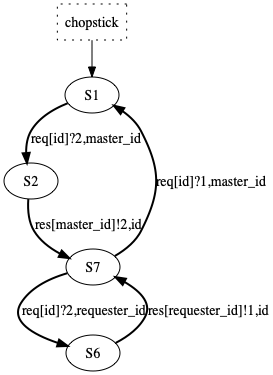
\includegraphics[width=0.3\textwidth]{chopstick}
\caption{گراف برنامهٔ نوع‌پردازهٔ \lr{chopstick}}
\end{figure}

\begin{figure}[H]
\centering
\begin{subfigure}[t]{0.4\textwidth}
    \centering
    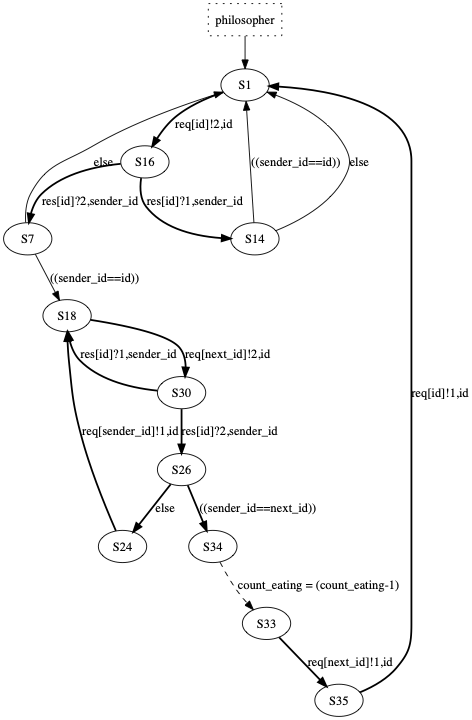
\includegraphics[width=\textwidth]{philosopher}
    \caption{نوع‌پردازهٔ \lr{philosopher}}
\end{subfigure}
~
\begin{subfigure}[t]{0.4\textwidth}
    \centering
    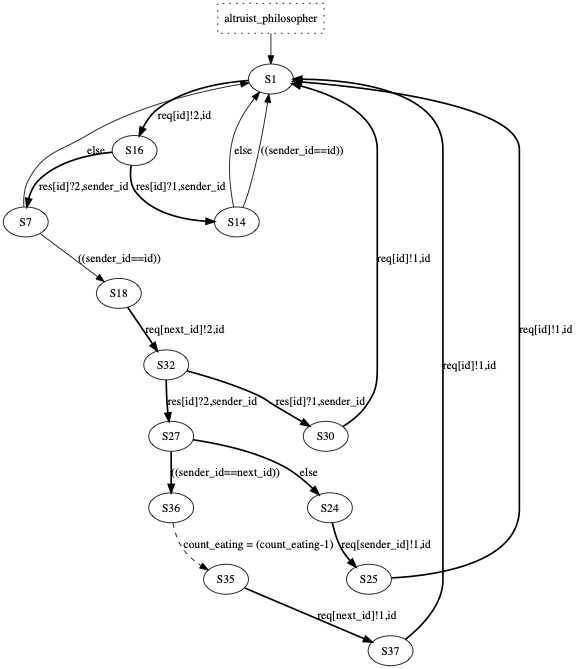
\includegraphics[width=\textwidth]{altruist_philosopher}
    \caption{نوع‌پردازهٔ \lr{altruist philosopher}}
\end{subfigure}
    \caption{گراف برنامهٔ نوع‌پردازه‌های \lr{philosopher}}
\end{figure}

\section{بررسی \lr{deadlock}}

مدل ارائه‌شده \lr{deadlock} ندارد اما سناریوهایی برای اجرای آن وجود دارد که پیشرفت (\lr{progress}) ندارند.

\begin{latin}
\small
\begin{verbatim}
(Spin Version 6.5.0 -- 1 July 2019)
    + Partial Order Reduction

Full statespace search for:
    never claim             - (none specified)
    assertion violations    +
    cycle checks        - (disabled by -DSAFETY)
    invalid end states  +

State-vector 192 byte, depth reached 9028, errors: 0
    55212 states, stored
   102737 states, matched
   157949 transitions (= stored+matched)
     1750 atomic steps
hash conflicts:       118 (resolved)
\end{verbatim}
\end{latin}

\section{بررسی حداقل طول کانال مورد نیاز}

برای کانال‌های پاسخ به فیلسوف‌ها (کانال‌های \lr{\lstinline|res|}) طول ۱ نیز کافی است.
برای کانال‌های درخواست به چوب‌های غذاخوری (کانال‌های \lr{\lstinline|req|}) حداقل طول ۲ ($n - 1$) مورد نیاز است.
برای بررسی این موضوع، از تعدادی \lr{\lstinline|assertion|} استفاده شد.

سناریوی زیر یک مثال است که نیاز به طول $n - 1$ را در کانال‌های \lr{\lstinline|req|} نشان می‌دهد.

\begin{latin}
\small
\begin{verbatim}
spin: phil-async.pml:33, Error: assertion violated
spin: text of failed assertion: assert((len(req[id])<max_len))
spin: trail ends after 58 steps
#processes: 13
        count_eating = 0
        queue 1 (req[0]): [release,2][request,2][request,0]
        queue 2 (req[1]): 
        queue 3 (req[2]): 
        queue 4 (res[0]): 
        queue 5 (res[1]): [forbid,2]
        queue 6 (res[2]): 
 58:    proc 12 (check_res_buffer_len:1) phil-async.pml:39 (state 3)
 58:    proc 11 (check_req_buffer_len:1) phil-async.pml:31 (state 3)
 58:    proc 10 (check_res_buffer_len:1) phil-async.pml:39 (state 3)
 58:    proc  9 (check_req_buffer_len:1) phil-async.pml:31 (state 3)
 58:    proc  8 (check_res_buffer_len:1) phil-async.pml:39 (state 3)
 58:    proc  7 (check_req_buffer_len:1) phil-async.pml:35 (state 4) <valid end state>
 58:    proc  6 (chopstick:1) phil-async.pml:96 (state 7)
 58:    proc  5 (altruist_philosopher:1) phil-async.pml:128 (state 32)
 58:    proc  4 (chopstick:1) phil-async.pml:96 (state 7)
 58:    proc  3 (philosopher:1) phil-async.pml:68 (state 30)
 58:    proc  2 (chopstick:1) phil-async.pml:96 (state 7)
 58:    proc  1 (philosopher:1) phil-async.pml:50 (state 16)
 58:    proc  0 (:init::1) phil-async.pml:27 (state 20) <valid end state>
13 processes created
\end{verbatim}
\end{latin}

\begin{figure}[H]
\centering
\includegraphics[width=\textwidth]{chan.pdf}
\caption{نمونه‌ای از اجرای نیازمند کانال‌های \lr{\lstinline|req|} با طول $n-1$}
\end{figure}

\end{document}
